\chapter{Algorithmic Approaches to Obtain Faithful Clustering}
In this chapter we have a closer look at the algorithms we designed and how they work.
We begin with \cref{sec:Encodings}, where we define the Boolean encodings for the semantics. Next, we described in \cref{sec:AlgorithmCheckingFaithfulness} how we decide if an AF is spurious or faithful. In \cref{sec:ConcretizingSingletons} we explain the concretization of a clustered argument. Next, in \cref{sec:ComputationOfConcretizerList} we explain how the concretizer list (a list of clustered arguments which are transformed to singletons) is computed. The approach to compute faithful abstract AFs is then described in \cref{sec:AlgorithmicApproachToComputeFaifthulClusterings}. Then we state the heuristics and refinements in \cref{sec:HeuristicsAndRefinements} and finally we discuss a specific relation between spurious sets in \cref{sec:AlgorithmsRelationsBetweenSpuriousSets}.


\section{Boolean Encodings for Abstract Semantics}
\label{sec:Encodings}
We previously defined the semantics in mathematical notation. But since we use SAT-Solving to compute extensions under a chosen semantics we develop in this section encodings in Boolean logic of the semantics of abstract AFs. We develop these encodings for (abstract) conflict-free, (abstract) admissible, and (abstract) stable extensions. For each semantics we present the corresponding Boolean encoding and an example.

In general, given an AF $\hat{G}=(\hat{A}, \hat{R})$, we will use Boolean variables corresponding to arguments. That is, if $a \in \hat{A}$ is an argument, then $a$ is also a Boolean variable. The intended meaning is then that in a truth-value assignment a variable $a$ is \emph{true}, then there is a corresponding set of arguments with $a$ in the set. Formally, if $\tau$ is a truth-value assignment on the variables in $\hat{A}$, then the corresponding set of arguments is defined as $\{a \in A \mid \tau(a) = 1\}$, where $1$ is the numerical equivalent to the Boolean \emph{true}.

We further define a subset of arguments, denoted as $\hat{A}_{\mathit{Single}} \subseteq \hat{A}$ consisting of the singletons arguments of the AF $G$, which effectively excludes each cluster.


\paragraph{Conflict-Free} We begin with (abstract) conflict-free sets. Recall that a set of (clustered) arguments is conflict-free if there is no attack between singletons in the set. Thus, the empty set is always part of the conflict-free sets.
\begin{definition}
    Let $\hat{G}=(\hat{A},\hat{R})$ be an abstract AF. Define the following formula.
        \[ \varphi_{cf}(\hat{G}) =
        \bigwedge_{a \in \hat{A}_{\mathit{Single}}} \bigl( \bigwedge_{b:(b,a)\in \hat{R}, b \in \hat{A}_{\mathit{Single}}} \lnot \bigl( a \wedge b \bigl) \bigl)
        \]
    \label{def:booleanFormulaConflictFree}
\end{definition}


\begin{example}
    Let us have a look at an example and define the abstract AF $\hat{G} = (\hat{A}, \hat{R})$ to be the AF depicted in \cref{af:algorithmEncodingsConflictFree}. With the arguments $\hat{A}=\{a, b, c, d\}$ and the attacks $\hat{R}=\big\{ (a,a)$, $(a,b)$, $(b,c)$, $(d,a)$, $(d,b)$, $(d,c)\big\}$.

    \begin{figure}[H]
        \centering
        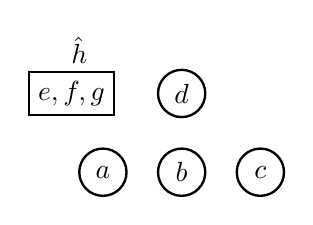
\begin{tikzpicture}
            % Singletons
            \def \ax{0}   \def \ay{-1}
            \def \bx{1}   \def \by{-1}
            \def \cx{2}   \def \cy{-1}
            \def \dx{1}   \def \dy{0}
            \def \hx{-0.4}    \def \hy{0}

            \draw[line width=0.3mm] (\ax, \ay) circle (0.3) node[anchor=center]{$a$};
            \draw[line width=0.3mm] (\bx, \by) circle (0.3) node[anchor=center]{$b$};
            \draw[line width=0.3mm] (\cx, \cy) circle (0.3) node[anchor=center]{$c$};
            \draw[line width=0.3mm] (\dx, \dy) circle (0.3) node[anchor=center]{$d$};
            \node[rectangle, draw, line width=0.3mm] at (\hx, \hy) {$e, f, g$};
            \node at (\hx + 0.1, \hy+0.55) {$\hat{h}$};

            % AttacksinproceedingsBesnardDoutreBooleanFormulaSemantics
            \DrawAttackHorizontal{R}{\ax}{\ay}{\bx}{\by}
            \DrawAttackHorizontal{R}{\bx}{\by}{\cx}{\cy}
            \DrawAttackHorizontal{B}{\dx}{\dy}{\hx+0.3}{\hy}
            \DrawSelfAttackLeftSingleton{\ax}{\ay}
            \DrawAttackDiagonal{PRL}{\dx}{\dy}{\ax}{\ay}
            \DrawAttackDiagonal{NLR}{\dx}{\dy}{\cx}{\cy}
            \DrawAttackVertical{D}{\dx}{\dy}{\bx}{\by}
        \end{tikzpicture}
        \caption{Abstract AF $\hat{G}$}
        \label{af:algorithmEncodingsConflictFree}
    \end{figure}

With \cref{def:booleanFormulaConflictFree} we obtain the following Boolean formula.
\begin{align*}
    \varphi_{cf}(\hat{G}) =\ &
    \lnot(b \land a)  \land
    \lnot(b \land d)  \land
    \lnot(a \land d)  \land
    \lnot(a \land a)  \land
    \\
    & \lnot(c \land b)  \land
    \lnot(c \land d)
\end{align*}

The models (i.e\ sets of variables assigned to true) of $\varphi_{cf}(\hat{G})$ in this example are $\bigl\{\emptyset$, $\{b\}$, $\{c\}$, $\{d\}$, $\{\hat{h}\}$, $\{b, \hat{h}\}$, $\{c, \hat{h}\}$, $\{d, \hat{h}\}\bigl\}$.
\end{example}

If we compare the models of $\varphi_{cf}(\hat{G})$ with the conflict-free sets of $\hat{G}$, we can observe that they are equal. In fact, \cref{def:booleanFormulaConflictFree} is a Boolean representation to obtain conflict-free sets from an AF. The formula can be applied to concrete and abstract AFs, because if no cluster is present, the formula corresponds to the previously defined conflict-free formula and only adds the layer of abstraction if at least one cluster is present \cite{inproceedingsBesnardDoutreBooleanFormulaSemantics}.


\paragraph{Admissible} Next we continue with (abstract) admissible sets. Recall that a set of arguments is abstractly admissible, if it is abstractly conflict-free and if every singleton which is being attacked, has a defender. For admissibility, the empty set does always satisfy the criteria and therefore is part of the admissible sets.

\begin{definition}
    Let $\hat{G}=(\hat{A}, \hat{R})$ be an abstract AF. Define the following formula.
        \[ \varphi_{adm}(\hat{G})=
        \varphi_{cf}(\hat{G}) \land  \bigwedge_{a \in \hat{A}_{\mathit{Single}}} \big( a \rightarrow \bigwedge_{b:(b,a) \in \hat{R}} \big( \bigvee_{c:(c,b) \in \hat{R}} c\big) \big)
        \]
    \label{def:booleanFormulaAdmissible}
\end{definition}


\begin{example}
    Let us have a look at an example and define the AF $\hat{G}=(\hat{A},\hat{R})$ to be the AF depicted in \cref{af:algorithmEncodingsAdmissible}. Where the arguments are $\hat{A}=\{a, b, c, d, e\}$ and the attacks $\hat{R}=\big\{ (a,a), (a,b), (b,c), (d,a), (d,b), (d,d), (d, e), (e, d)\big\}$.

    \begin{figure}[H]
        \centering
        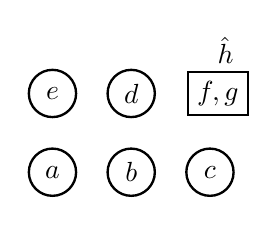
\begin{tikzpicture}
            % Singletons
            \def \ax{0}   \def \ay{-1}
            \def \bx{1}   \def \by{-1}
            \def \cx{2}   \def \cy{-1}
            \def \dx{1}   \def \dy{0}
            \def \ex{0}   \def \ey{0}
            \def \hx{2.1}    \def \hy{0}

            \draw[line width=0.3mm] (\ax, \ay) circle (0.3) node[anchor=center]{$a$};
            \draw[line width=0.3mm] (\bx, \by) circle (0.3) node[anchor=center]{$b$};
            \draw[line width=0.3mm] (\cx, \cy) circle (0.3) node[anchor=center]{$c$};
            \draw[line width=0.3mm] (\dx, \dy) circle (0.3) node[anchor=center]{$d$};
            \draw[line width=0.3mm] (\ex, \ey) circle (0.3) node[anchor=center]{$e$};
            \node[rectangle, draw, line width=0.3mm] at (\hx, \hy) {$f, g$};
            \node at (\hx + 0.1, \hy+0.55) {$\hat{h}$};

            % Attacks
            \DrawAttackHorizontal{R}{\ax}{\ay}{\bx}{\by}
            \DrawAttackHorizontal{R}{\bx}{\by}{\cx}{\cy}
            \DrawAttackHorizontal{B}{\dx}{\dy}{\ex}{\ey}
            
            \DrawAttackVertical{B}{\hx-0.1}{\hy}{\cx}{\cy}

            \DrawSelfAttackLeftSingleton{\ax}{\ay}
            \DrawSelfAttackRightSingleton{\dx}{\dy}
            \DrawAttackDiagonal{PRL}{\dx}{\dy}{\ax}{\ay}
            \DrawAttackVertical{D}{\dx}{\dy}{\bx}{\by}
        \end{tikzpicture}
        \caption{Abstract AF $\hat{G}$}
        \label{af:algorithmEncodingsAdmissible}
    \end{figure}

By applying the formula defined in \cref{def:booleanFormulaAdmissible} to the AF $\hat{G}$, we obtain the following Boolean expression.
\begin{align*}
    \varphi_{adm}(\hat{G}) = &\big(
     \lnot (a \land a) \land \lnot (a \land d) \land \lnot (b \land d) \land \lnot (b \land c) \land \lnot (b \land d) \land \lnot (c \land b) \land \lnot (d \land e) \land \\
      & \lnot (d \land d) \land \lnot (e \land d) \big) \land\\
      &\bigl( a \rightarrow ((a \lor d) \land (e \lor d)) \land \bigl( b \rightarrow ((a \lor d) \land (b) \land (e \lor d)) \bigl) \bigl) \land\\
      &\bigl( c \rightarrow ((a \lor c \lor d) \land (\hat{h})) \bigl) \land \bigl( d \rightarrow (d) \land (e \lor d) \bigl) \land \bigl( e \rightarrow (e \lor d) \bigl)
\end{align*}

The models of $\varphi_{adm}(\hat{G})$ in this example are $\big\{\emptyset$, $\{c\}$, $\{e\}$, $\{\hat{h}\}$, $\{c, e\}$, $\{c, \hat{h}\}$, $\{e, \hat{h}\}$, $\{c, e, \hat{h}\} \big\}$.
\end{example}

If we compare the models of $ \varphi_{adm}(\hat{G})$ with the admissible sets of $\hat{G}$, we can observe that they are equal. Indeed, \cref{def:booleanFormulaAdmissible} provides a Boolean representation that allows the derivation of admissible sets from an AF. If the AF $\hat{G}$ has no cluster, the formula reduces a previously defined formula for admissible sets \cite{inproceedingsBesnardDoutreBooleanFormulaSemantics}.



\paragraph{Stable} Finally we take a look at the (abstract) stable extensions. Recall, that a set of arguments is abstractly stable, if it is abstractly conflict-free and if an
argument is not in the abstractly stable extension, it implies that an argument in the
abstractly stable extension is attacking it. Furthermore if the abstractly stable extension
is not attacking an argument, then every singleton attacked by the argument is not in the
abstractly stable extension. Other than conflict-free and admissible, the empty set is not a stable extension except if $\hat{A} = \emptyset$.
\begin{definition}
    Let $\hat{G}=(\hat{A},\hat{R})$ be an abstract AF. Define the following formula.
        \[ \varphi_{stb}(\hat{G}) =
        \varphi_{cf}(\hat{G}) \land \bigwedge_{a \in \hat{A}} \big( a \bigvee_{b:(b,a)\in \hat{R}} b\big) \land \bigwedge_{a \in \hat{A}} \big( \big(  a \bigwedge_{b:(b,a) \in \hat{R}} \lnot b\big)  \rightarrow \big( \bigwedge_{c:(a,c), c \in \hat{A}_{\mathit{Single}}} \lnot c\big) \big)
        \]
    \label{def:booleanFormulaStable}
\end{definition}


\begin{example}
    Let us have a look at an example and define the AF $\hat{G}=(\hat{A}, \hat{R})$ to be the abstract AF depicted in \cref{af:algorithmEncodingsStable}. Where the arguments are $\hat{A}=\{a, b, c, d\}$ and the attacks $\hat{R}=\big\{ (a,a)$, $(a,b)$, $(a,d)$, $(b,a)$, $(b,d)$, $(c,b)$, $(d,a)\big\}$.

    \begin{figure}[H]
        \centering
        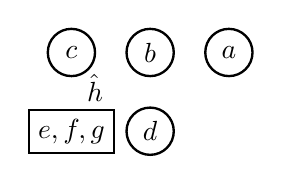
\begin{tikzpicture}
            % Singletons
            \def \ax{2}   \def \ay{0}
            \def \bx{1}   \def \by{0}
            \def \cx{0}   \def \cy{0}
            \def \dx{1}   \def \dy{-1}
            \def \hx{0}   \def \hy{-1}

            \draw[line width=0.3mm] (\ax, \ay) circle (0.3) node[anchor=center]{$a$};
            \draw[line width=0.3mm] (\bx, \by) circle (0.3) node[anchor=center]{$b$};
            \draw[line width=0.3mm] (\cx, \cy) circle (0.3) node[anchor=center]{$c$};
            \draw[line width=0.3mm] (\dx, \dy) circle (0.3) node[anchor=center]{$d$};
            \node[rectangle, draw, line width=0.3mm] at (\hx, \hy) {$e, f, g$};
            \node at (\hx + 0.3, \hy+0.55) {$\hat{h}$};
            % Attacks
            \DrawSelfAttackRightSingleton{\ax}{\ay}
            \DrawAttackHorizontal{R}{\cx}{\cy}{\bx}{\by}
            \DrawAttackHorizontal{B}{\ax}{\ay}{\bx}{\by}
            \DrawAttackVertical{D}{\bx}{\by}{\dx}{\dy}
            \DrawAttackVertical{D}{\cx}{\cy}{\hx}{\hy}
            \DrawAttackDiagonal{PLR}{\dx}{\dy}{\ax}{\ay}
        \end{tikzpicture}
        \caption{Abstract AF $\hat{G}$}
        \label{af:algorithmEncodingsStable}
    \end{figure}

If we apply the encoded formula defined in \cref{def:booleanFormulaStable} to the AF $\hat{G}$, we obtain the following Boolean expression.
\begin{align*}
    \varphi_{stb}(\hat{G}) = &\bigl( (\lnot (a \land a)) \land (\lnot (a \land b)) 
    \land (\lnot (b \land a)) \land (\lnot (b \land c)) \land (\lnot (d \land b)) \bigl) \land\\
    & \bigl( (a \lor a \lor b \lor d) \land (b \lor a \lor c) \land (d \lor b) \land (\hat{h} \lor c)\bigl) \land \\
    & \bigl( ((a \land \lnot a \land \lnot b \land \lnot d) \rightarrow (\lnot a \land \lnot b)\bigl) \land\\
    & \bigl((b \land \lnot a \land \lnot c) \rightarrow (\lnot a \land \lnot d)) \land ((d \land \lnot b) \rightarrow \lnot a)\bigl)
\end{align*}


The models of $\varphi_{stb}(\hat{G})$ in this example are $\bigl\{$$\{c, d\}$, $\{c, d, \hat{h}\} \bigl\}$.
\end{example}

By comparing the models of $\varphi_{stb}(\hat{G})$ with the stable sets of $\hat{G}$, we find that they are identical. Specifically, \cref{def:booleanFormulaStable} is a Boolean expression to derive stable sets from an AF. If the AF has no clusters, the Boolean expression reduces to the stable formula defined earlier.


\section{Checking Faithfulness}
\label{sec:AlgorithmCheckingFaithfulness}
In the context of abstract AFs, faithfulness is an important property. To be able to determine if an AF is faithful or spurious we develop two different approaches, i.e., BFS and DFS wich are described in \cref{subsec:BFSandDFSAlgorithm}. To be able to show faithfulness or spuriousness for a specific abstract extension, we developed again two different procedures, i.e., list comparison and the SAT-based check described in \cref{subsec:ExtensionMapping}.

\subsection{BFS and DFS}
\label{subsec:BFSandDFSAlgorithm}
Breadth-First-Search (BFS) and Depth-First-Search (DFS) are usually used in algorithms to traverse graphs. Where BFS visits each node in order of distance to the start, DFS follows a direct path and only backtracks, if it has to. We, however, are not using the two approaches to traverse a graph, but we are using a similar principle on the computation of semantics.

\paragraph{BFS} The BFS approach in our implementation, depicted in \cref{fig:ImplementationBFSVisualization}, first computes all the semantics extensions of the abstract AF and then checks if any of the extensions is spurious. After one spurious extension is encountered, the algorithm is aborted, because if one extension is spurious the AF is spurious as well.

The BFS approach is practical for AFs which do not have many semantics extensions. If the semantics sets take too long to compute, we will run into a timeout no matter at which seed the SAT-Solver is operating on. BFS is a solid and robust approach, nevertheless, there is no space of randomness and lucky early terminations.

\begin{figure}[h!]
    \centering
    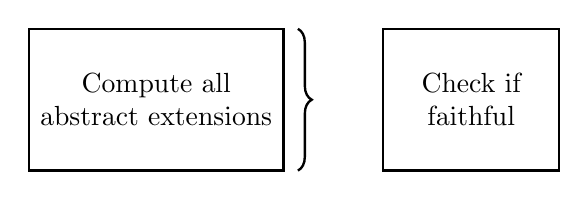
\begin{tikzpicture}
        % Compute Block
        \def \computeBlockX{0}
        \def \computeBlockY{0}
        \def \computeBlockWidth{3cm}
        \def \computeBlockHeight{1.8cm}
        \node[rectangle, draw, line width=0.3mm, minimum width=\computeBlockWidth, minimum height=\computeBlockHeight , text width=\computeBlockWidth, align=center] at (\computeBlockX, \computeBlockY) {Compute all abstract extensions};


        % Check Block
        \def \checkBlockX{4}
        \def \checkBlockY{0}
        \def \checkBlockWidth{2cm}
        \def \checkBlockHeight{1.8cm}
        \node[rectangle, draw, line width=0.3mm, minimum width=\checkBlockWidth, minimum height=\checkBlockHeight , text width=\checkBlockWidth, align=center] at (\checkBlockX, \checkBlockY) {Check if faithful};
        % Brace
        \draw [line width=0.3mm, decorate, decoration = {brace, amplitude=5pt, mirror}] (1.8, - \checkBlockHeight/2) --  (1.8, \checkBlockHeight/2);
        \DrawAttackHorizontal{R}{1.7}{0}{3.15}{0}
    \end{tikzpicture}
    \caption{BFS visualization}
    \label{fig:ImplementationBFSVisualization}
\end{figure}


\paragraph{DFS} On the other hand we have the DFS approach, depicted in \cref{fig:ImplementationDFSVisualization}. When using DFS, instead of calculating all the abstract extensions at once, we verify each computed set directly. Verifying in this context means, to check if the extension can be mapped to one of the concrete extensions. If an extension cannot be mapped, we found a spurious extension which shows spuriousness of the AF.

DFS has some overhead, due to the context switches resulting with a longer computation power for faithful AFs. Nevertheless, depending on the seed of the SAT-Solver, we can obtain a result much faster than with BFS. If the first computed semantics extension is already spurious, we save a lot of computation power and can even solve AFs, which are not feasible for the BFS approach.



\begin{figure}[h]
    \centering
    \begin{tikzpicture}
        \def \bwidth{3cm}
        \def \bheight{1.5cm}
        % Block 1
        \def \cbIX{0}
        \def \cbIY{1.1cm}
        \node[rectangle, draw, line width=0.3mm, minimum width=\bwidth, minimum height=\bheight , text width=\bwidth, align=center] at (\cbIX, \cbIY) {Compute abstract extension};

        % Block connection dotted
        \draw[densely dotted,-, line width=0.3mm, >={To[length=4, width=5]}]
        (\cbIX, 0.25cm) -- (\cbIX, -0.25cm);

        % Block 2
        \def \cbIIX{0}
        \def \cbIIY{-1.1cm}
        \node[rectangle, draw, line width=0.3mm, minimum width=\bwidth, minimum height=\bheight , text width=\bwidth, align=center] at (\cbIIX, \cbIIY) {Compute abstract extension};



        % Block 3
        \def \cbIIIX{4}
        \def \cbIIIY{1.1cm}
        \node[rectangle, draw, line width=0.3mm, minimum width=\bwidth, minimum height=\bheight , text width=\bwidth, align=center] at (\cbIIIX, \cbIIIY) {Check if faithful};
        \DrawAttackHorizontal{R}{1.3}{\cbIIIY}{2.7}{\cbIIIY}

        % Block connection dotted
        \draw[densely dotted,-, line width=0.3mm, >={To[length=4, width=5]}]
        (\cbIIIX, 0.25cm) -- (\cbIIIX, -0.25cm);

        % Block 4
        \def \cbIIIIX{4}
        \def \cbIIIIY{-1.1cm}
        \node[rectangle, draw, line width=0.3mm, minimum width=\bwidth, minimum height=\bheight , text width=\bwidth, align=center] at (\cbIIIIX, \cbIIIIY) {Check if faithful};
        \DrawAttackHorizontal{R}{1.3}{\cbIIIIY}{2.7}{\cbIIIIY}


        % Brace
        \draw [line width=0.3mm, decorate, decoration = {brace, amplitude=5pt, mirror}] (5.8,-1.85) --  (5.8,1.85);
        \DrawAttackHorizontal{R}{5.7}{0}{6.9}{0}

        % Check Block
        \def \checkBlockX{8}
        \def \checkBlockY{0}
        \def \checkBlockWidth{2.5cm}
        \def \checkBlockHeight{3.5cm}
        \node[rectangle, draw, line width=0.3mm, minimum width=\checkBlockWidth, minimum height=\checkBlockHeight , text width=\checkBlockWidth, align=center] at (\checkBlockX, \checkBlockY) {If any check is unsatisfiable, return spurious};
    \end{tikzpicture}
    \caption{DFS visualization}
    \label{fig:ImplementationDFSVisualization}
\end{figure}



\subsection{Extension Mapping}
\label{subsec:ExtensionMapping}
To determine if an abstract extension is faithful or spurious, we need to map it to a concrete extension. If this is not possible, we found a spurious extension. We created two procedures for the mapping, i.e., list comparison and SAT-Based check.

\paragraph{List Comparison}
The first approach of mapping an abstract extension to a concrete extension is the list comparison. Here, all the concrete extensions are computed and are then checked iteratively for the mapping. Since list comparisons are highly optimized and do not need an additional SAT-Solver invocation, the approach can be efficient under certain circumstances.

The issue with the list comparison of the computed extension is, that for AFs with big clusters (i.e.\ a cluster containing many arguments), the direct mapping of an abstract extension is tedious. This is because of the many possibilities a cluster can transform into, e.g., for a cluster $\hat{h}$ containing the arguments $a$ and $b$, the extension $\{\hat{h}\}$ could transformed into $\{a\}$, $\{b\}$ and $\{a, b\}$. This works fine for small clusters, but can be become more computationally intensive for larger clusters.


\paragraph{SAT-Based check}
For optimization reasons, we altered the way on how to check for faithfulness. That is, why we implemented a SAT-based check. Instead of computing the concrete extensions, we check if the formula of the semantics from the concrete AF is still satisfiable, if we add the abstract extension. The abstract extension is encoded with the corresponding Boolean variables, where every argument in the extension is set to \emph{true} and the arguments not in the extension is set to \emph{false}. The clusters are enrolled by the clustered arguments disjunctively, to cover every possible cluster mapping.





\section{Concretizing Singletons}
\label{sec:ConcretizingSingletons}
When operating on abstract AFs, a crucial transformation is to extract arguments from a cluster and transform it to a singleton. This is called concretizing. When clustering singletons, the cluster inherits the attacks of the argument, concretizing is the inverse operation. This means, that it needs to revert the changes done by the clustering. Since clustering does not preserve all the information, i.e.\ the attacks directed towards and originating from the clustered arguments, the abstraction does lead to a loss of details. To be able to concretize argument, this needs to compensate by providing additionally the concrete AF. With the concrete AF we can reconstruct the attacks of the arguments and transform the AF in such a way, as if it was primarily abstracted the same manner, but without the arguments intended to be concretized.

Concretizing a list of arguments is done iteratively by duplicating the abstract AF $\hat{F}$ to create a new AF $\hat{F}'$ and transforming it. The transformation is guided by five steps considering the unchanged abstract AF $\hat{F}$ and the concrete AF $F$. To improve the understanding of each step, we accompany the explanation with the example depicted in \cref{example:concretizationOfArguments}, where we concretize the arguments $a$ and $b$.


\vspace{0.3cm}
\begin{figure}[h]
    \centering
    \begin{subfigure}[t]{0.45\textwidth}
        \centering
        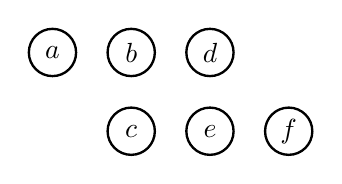
\begin{tikzpicture}
            % Singletons
                \def \ax{0}   \def \ay{0}
                \def \bx{1}   \def \by{0}
                \def \cx{1}   \def \cy{-1}
                \def \dx{2}   \def \dy{0}
                \def \ex{2}   \def \ey{-1}
                \def \fx{3}   \def \fy{-1}

                \draw[line width=0.3mm] (\ax, \ay) circle (0.3) node[anchor=center]{$a$};
                \draw[line width=0.3mm] (\bx, \by) circle (0.3) node[anchor=center]{$b$};
                \draw[line width=0.3mm] (\cx, \cy) circle (0.3) node[anchor=center]{$c$};
                \draw[line width=0.3mm] (\dx, \dy) circle (0.3) node[anchor=center]{$d$};
                \draw[line width=0.3mm] (\ex, \ey) circle (0.3) node[anchor=center]{$e$};
                \draw[line width=0.3mm] (\fx, \fy) circle (0.3) node[anchor=center]{$f$};
                % Attacks
                \DrawAttackHorizontal{L}{\bx}{\by}{\ax}{\ay}
                \DrawAttackHorizontal{L}{\dx}{\dy}{\bx}{\by}

                \DrawAttackVertical{D}{\bx}{\by}{\cx}{\cy}
                \DrawAttackVertical{U}{\ex}{\ey}{\dx}{\dy}

                \DrawAttackDiagonal{NRL}{\cx}{\cy}{\ax}{\ay}
        \end{tikzpicture}
        \subcaption{Concrete AF $F$}
        \label{fig:concrete_af}
    \end{subfigure}%
    \hfill
    \begin{subfigure}[t]{0.55\textwidth}
        \centering
        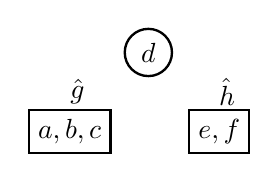
\begin{tikzpicture}
            % Singletons
            \def \dx{1}   \def \dy{0}
            \def \gx{0}   \def \gy{-1}
            \def \hx{1.9}   \def \hy{-1}
            \draw[line width=0.3mm] (\dx, \dy) circle (0.3) node[anchor=center]{$d$};
            % Cluster
            \node[rectangle, draw, line width=0.3mm] at (\gx, \gy) {$a,b,c$};
            \node at (\gx + 0.1, \gy+0.5) {$\hat{g}$};
            \node[rectangle, draw, line width=0.3mm] at (\hx, \hy) {$e,f$};
            \node at (\hx + 0.1, \hy+0.5) {$\hat{h}$};
            % Attacks
            \DrawAttackDiagonal{PRL}{\dx}{\dy}{\gx+0.1}{\gy+0.1}
            \DrawAttackDiagonal{NRL}{\hx}{\hy+0.1}{\dx}{\dy}
            \DrawSelfAttackLeftTopCluster{\gx-0.45}{\gy+0.3}
        \end{tikzpicture}
        \subcaption{Abstract AF $\hat{F}$}
        \label{fig:abstract_af}
    \end{subfigure}
    \caption{Concrete and abstract AF}
    \label{example:concretizationOfArguments}
\end{figure}


\paragraph{Step 1:} Each argument needing concretization is first removed from the parent cluster and added as a singleton in $\hat{F}'$ with no attacks towards or originating from the singleton. If an argument is not part of a cluster, we ignore it and remove it from the list of arguments to be concretized.
We do not consider attacks in this step since they depend on the concrete- and abstract AFs which we will consider on the next step. The resulting AF is depicted in \cref{example:algorithmConcretizeSingletonsStep1} and the pseudo-code in \cref{alg:concretizingSingletonsStep1}. We defined the arguments to be concretized as a list of arguments $list(S)$, with $S$ being the computed concretizer list. Furthermore, we have an AF datastructure $F: AF(A, R)$. Here $A$ is a dictionary of arguments, where each argument has the property $attacks$ (i.e.\ a list of arguments that are being attacked by the argument) and $attacked\_by$ (i.e.\ a list of arguments that attack the argument). The attacks of the AF are stored in the list $R$, where the entities of an attack $r=(a, b)$ can be extracted with $r.source$, mapping to the attacker $a$ of the attack $r$ and $r.target$, mapping to the argument that is being attacked $b$ in the attack $r$.


\vspace{0.3cm}
\begin{figure}[h]
    \centering
    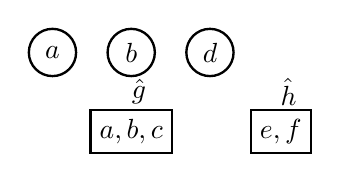
\begin{tikzpicture}
        % Singletons
        \def \ax{0}   \def \ay{0}
        \def \bx{1}   \def \by{0}
        \def \dx{2}   \def \dy{0}
        \def \gx{1}   \def \gy{-1}
        \def \hx{2.9}   \def \hy{-1}

        \draw[line width=0.3mm] (\ax, \ay) circle (0.3) node[anchor=center]{$a$};
        \draw[line width=0.3mm] (\bx, \by) circle (0.3) node[anchor=center]{$b$};
        \draw[line width=0.3mm] (\dx, \dy) circle (0.3) node[anchor=center]{$d$};
        % Cluster

        \node[rectangle, draw, line width=0.3mm] at (\gx, \gy) {$a,b,c$};
        \node at (\gx + 0.1, \gy + 0.5) {$\hat{g}$};

        \node[rectangle, draw, line width=0.3mm] at (\hx, \hy) {$e,f$};
        \node at (\hx + 0.1, \hy + 0.5) {$\hat{h}$};

        % Attacks
        \DrawAttackDiagonal{PRL}{\dx}{\dy}{\gx+0.1}{\gy+0.1}
        \DrawAttackDiagonal{NRL}{\hx}{\hy+0.1}{\dx}{\dy}
        \DrawSelfAttackLeftTopCluster{\gx-0.45}{\gy+0.3}

    \end{tikzpicture}
    \caption{Concretized AF $\hat{F}'$ after Step 1}
    \label{example:algorithmConcretizeSingletonsStep1}
\end{figure}
\vspace{-0.2cm}


\begin{algorithm}[H]
    \caption{Concretizing Singletons Pseudocode Step 1}\label{alg:concretizingSingletonsStep1}
    \begin{algorithmic}[1]
        \Require $\hat{F}: AF(\hat{A}, \hat{R})$ \Comment{Abstract Clustered AF}
        \Require $e: list(S)$ \Comment{Concretizer List}
        \State $\hat{F}'$ $\gets$ $\hat{F}$ \Comment{$N$ = Concretized Cluster}
        \For{$a_i$ in $e$}
            \For{$c_i$ in $\hat{F}.clusters$}
                \If{$a_i$ in $c_i$}
                    \State $c_i.remove(a_i)$
                \EndIf
                \EndFor
            \State $\hat{F}'.addSingleton(a_i)$
        \EndFor
    \end{algorithmic}
\end{algorithm}




\paragraph{Step 2:} We add the new attacks from all concretized arguments to the remaining clusters and vice versa. We must do this after removing the arguments from the clusters because if an argument $a$ attacks argument $b$ in the concrete AF $F$, and $b$ is part of the cluster $\hat{g}$ in the abstract AF $\hat{F}$, by concretizing $b$, the attack $(a,\hat{g})$ would not be present anymore. The resulting AF $\hat{F}'$ is depicted in \cref{example:algorithmConcretizeSingletonsStep2} and the pseudo-code in \cref{alg:concretizingSingletonsStep2}. The pseudo code iterates over all the arguments to be concretized and adds the missing attacks from the clusters to the arguments and vice versa.


\vspace{0.3cm}
\begin{figure}[h]
    \centering
    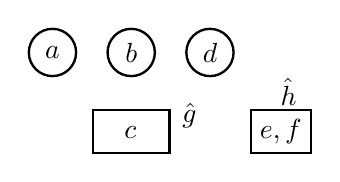
\begin{tikzpicture}
        % Singletons
        \def \ax{0}   \def \ay{0}
        \def \bx{1}   \def \by{0}
        \def \dx{2}   \def \dy{0}
        \def \gx{1}   \def \gy{-1}
        \def \hx{2.9}   \def \hy{-1}

        \draw[line width=0.3mm] (\ax, \ay) circle (0.3) node[anchor=center]{$a$};
        \draw[line width=0.3mm] (\bx, \by) circle (0.3) node[anchor=center]{$b$};
        \draw[line width=0.3mm] (\dx, \dy) circle (0.3) node[anchor=center]{$d$};
        % Cluster

        \node[rectangle, draw, line width=0.3mm] at (\gx, \gy) {$\phantom{a,} c\phantom{, b}$};
        \node at (\gx + 0.74, \gy + 0.2) {$\hat{g}$};

        \node[rectangle, draw, line width=0.3mm] at (\hx, \hy) {$e,f$};
        \node at (\hx + 0.1, \hy + 0.5) {$\hat{h}$};

        % Attacks
        \DrawAttackDiagonal{PRL}{\dx}{\dy}{\gx+0.1}{\gy+0.1}
        \DrawAttackDiagonal{NRL}{\hx}{\hy+0.1}{\dx}{\dy}
        \DrawSelfAttackLeftTopCluster{\gx-0.45}{\gy+0.3}
        \DrawAttackVertical{D}{\bx}{\by}{\gx}{\gy}
        \DrawAttackDiagonal{NRL}{\gx-0.1}{\gy+0.1}{\ax}{\ay}


    \end{tikzpicture}
    \caption{Concretized AF $\hat{F}'$ after Step 2}
    \label{example:algorithmConcretizeSingletonsStep2}
\end{figure}
\vspace{-0.2cm}



\begin{algorithm}[H]
    \caption{Concretizing Singletons Pseudocode Step 2}\label{alg:concretizingSingletonsStep2}
    \begin{algorithmic}[1]
        \Require $F: AF(A, R)$ \Comment{Concrete AF}
        \Require $e: list(S)$ \Comment{Concretizer List}
        \Require $\hat{F}': AF(\hat{A}', \hat{R}')$ \Comment{Concretized Cluster}
        \For{$e_i$ in $e$}
            \For{$att_i$ in $F[e_i].attacks$} \Comment{Add attacks (argument, cluster)}
                \If{$att_i$ is cluster}
                    \State $\hat{F}'.addAttack((e_i, att_i))$
                \EndIf
            \EndFor
            \For{$att\_by_i$ in $F[e_i].attacked\_by$} \Comment{Add attacks (cluster, argument)}
                \If{$att\_by_i$ is cluster}
                    \State $\hat{F}'.addAttack((att\_by_i, e_i))$
                \EndIf
            \EndFor
        \EndFor
    \end{algorithmic}
\end{algorithm}



\paragraph{Step 3:} After adding the new attacks, we need to check which attacks from $\hat{F}$ are still present in $\hat{F}'$. If an attack does not persist through the concretization, we remove it in $\hat{F}'$. An attack is not present anymore if we remove one of the arguments being attacked or attacked by argument $a$ from a cluster $\hat{f}$ and no other attack exists, s.t. $a$ is attacked from/attacking an argument within $\hat{f}$. Selfattacks of clusters could also change by the concretization of arguments. Therefore, we need to check the clusters from which the arguments are concretized. The resulting AF is depicted in \cref{example:algorithmConcretizeSingletonsStep3} and the pseudo-code in \cref{alg:concretizingSingletonsStep3}.

To add further explanation of the pseudo-code, we split the code into three parts. All of them are encased in a iteration over all the attacks of the abstract AF. In each step we cover a different case of the entities from the current attack $(a, b)$.
In the first part, we check if both entities $a$ and $b$ are clusters. If so, we check if any clustered argument from the attacker cluster $a$ attacks any clustered argument of the cluster $b$ in the concrete AF. If no attack is found, we remove the current attack $(a, b)$ from the concretized AF.
The second part covers the case, when the attacker $a$ is a singleton and the defender $b$ is a cluster. In this case, we check if $a$ attacks any of the clustered arguments from $b$ in the concrete AF. If this does not hold, we remove the attack $(a, b)$ from the concretized AF.
And finally, the third part covers the case, if the attacker $a$ is a cluster and the defender $b$ is a singleton. Here we do the same as in the second part, but with $a$ and $b$ reversed.

\vspace{0.3cm}
\begin{figure}[h]
    \centering
    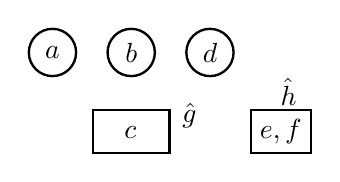
\begin{tikzpicture}
        % Singletons
        \def \ax{0}   \def \ay{0}
        \def \bx{1}   \def \by{0}
        \def \dx{2}   \def \dy{0}
        \def \gx{1}   \def \gy{-1}
        \def \hx{2.9}   \def \hy{-1}

        \draw[line width=0.3mm] (\ax, \ay) circle (0.3) node[anchor=center]{$a$};
        \draw[line width=0.3mm] (\bx, \by) circle (0.3) node[anchor=center]{$b$};
        \draw[line width=0.3mm] (\dx, \dy) circle (0.3) node[anchor=center]{$d$};
        % Cluster

        \node[rectangle, draw, line width=0.3mm] at (\gx, \gy) {$\phantom{a,} c\phantom{, b}$};
        \node at (\gx + 0.74, \gy + 0.2) {$\hat{g}$};

        \node[rectangle, draw, line width=0.3mm] at (\hx, \hy) {$e,f$};
        \node at (\hx + 0.1, \hy + 0.5) {$\hat{h}$};

        % Attacks
        \DrawAttackDiagonal{NRL}{\hx}{\hy+0.1}{\dx}{\dy}
        \DrawAttackVertical{D}{\bx}{\by}{\gx}{\gy}
        \DrawAttackDiagonal{NRL}{\gx-0.1}{\gy+0.1}{\ax}{\ay}
    \end{tikzpicture}
    \caption{Concretized AF $\hat{F}'$ after Step 3}
    \label{example:algorithmConcretizeSingletonsStep3}
\end{figure}
\vspace{-0.2cm}

\begin{algorithm}[H]
    \caption{Concretizing Singletons Pseudocode Step 3}\label{alg:concretizingSingletonsStep3}
    \begin{algorithmic}[1]
        \Require $F: AF(A, R)$ \Comment{Concrete AF}
        \Require $\hat{F}: AF(\hat{A}, \hat{R})$ \Comment{Abstract AF}
        \Require $\hat{F}': AF(\hat{A}', \hat{R}')$ \Comment{Concretized Cluster}
        \For{$r_i$ in $\hat{R}'$}
            \If{$r_i.target$ is cluster and $r_i.source$ is cluster} \Comment{Part 1}
                \For{$a_i$ in $\hat{F}[r_i.source]$}
                    \If{\textbf{not}($a_i$ attacks any of $A[r_i.target]$)}
                        \State $\hat{F}'.removeAttack(r_i)$
                        \State break
                    \EndIf
                \EndFor
            \EndIf
            \If{$r_i.target$ is cluster} \Comment{Part 2}
                \If{\textbf{not}($r_i.source$ attacks any of $A[r_i.target]$)}
                    \State $\hat{F}'.removeAttack(r_i)$
                    \State continue
                \EndIf
            \EndIf
            \If{$r_i.source$ is cluster} \Comment{Part 3}
                \If{\textbf{not} ($r_i.target$ is attacked by any $A[r_i.source]$)}
                    \State $\hat{F}'.removeAttack(r_i)$
                    \State continue
                \EndIf
            \EndIf
        \EndFor
    \end{algorithmic}
\end{algorithm}


\paragraph{Step 4:} In this step we add the new attacks between the singletons. Due to the fact that we copied all the attacks from $\hat{F}$, we only have to take into consideration the attacks towards or originating to the concretized singletons. So instead of iterating over all singletons of the AF $\hat{F}'$, we can limit the attack creation to the concretized singletons. The resulting AF is depicted in \cref{example:algorithmConcretizeSingletonsStep4} and the pseudo-code in \cref{alg:concretizingSingletonsStep4}. To explain the pseudo-code a bit further, we iterate over all the arguments which need to be concretized and check their direct defender and attacker from the concrete AF and then add the missing attacks to the concretized AF.


\vspace{0.3cm}
\begin{figure}[h]
    \centering
    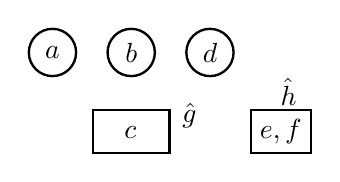
\begin{tikzpicture}
        % Singletons
        \def \ax{0}   \def \ay{0}
        \def \bx{1}   \def \by{0}
        \def \dx{2}   \def \dy{0}
        \def \gx{1}   \def \gy{-1}
        \def \hx{2.9}   \def \hy{-1}

        \draw[line width=0.3mm] (\ax, \ay) circle (0.3) node[anchor=center]{$a$};
        \draw[line width=0.3mm] (\bx, \by) circle (0.3) node[anchor=center]{$b$};
        \draw[line width=0.3mm] (\dx, \dy) circle (0.3) node[anchor=center]{$d$};
        % Cluster

        \node[rectangle, draw, line width=0.3mm] at (\gx, \gy) {$\phantom{a,} c\phantom{, b}$};
        \node at (\gx + 0.74, \gy + 0.2) {$\hat{g}$};

        \node[rectangle, draw, line width=0.3mm] at (\hx, \hy) {$e,f$};
        \node at (\hx + 0.1, \hy + 0.5) {$\hat{h}$};

        % Attacks
        \DrawAttackDiagonal{NRL}{\hx}{\hy+0.1}{\dx}{\dy}
        \DrawAttackVertical{D}{\bx}{\by}{\gx}{\gy}
        \DrawAttackDiagonal{NRL}{\gx-0.1}{\gy+0.1}{\ax}{\ay}
        \DrawAttackHorizontal{L}{\dx}{\dy}{\bx}{\by}
        \DrawAttackHorizontal{L}{\bx}{\by}{\ax}{\ay}
    \end{tikzpicture}
    \caption{Concretized AF $\hat{F}'$ after Step 4}
    \label{example:algorithmConcretizeSingletonsStep4}
\end{figure}
\vspace{-0.2cm}


\begin{algorithm}[H]
    \caption{Concretizing Singletons Pseudocode Step 4}\label{alg:concretizingSingletonsStep4}
    \begin{algorithmic}[1]
        \Require $F: AF(A, R)$ \Comment{Concrete AF}
        \Require $\hat{F}: AF(\hat{A}, \hat{R})$ \Comment{Abstract AF}
        \Require $\hat{F}': AF(\hat{A}', \hat{R}')$ \Comment{Concretized Cluster}
        \Require $e: list(S)$ \Comment{Concretizer List}
        \For{$e_i$ in $e$}
            \For{$a_i$ in $A[e_i.attacks]$}
                \If{$a_i$ is singleton and ($e_i$, $a_i$) not in $R$}
                    \State $\hat{F}'.addAttack((e_i, a_i))$
                \EndIf
            \EndFor
            \For{$a_i$ in $A[e_i.attacked\_by]$}
                \If{$a_i$ is singleton and ($a_i$, $e_i$) not in $R$}
                    \State $\hat{F}'.addAttack((a_i, e_i))$
                \EndIf
            \EndFor
        \EndFor
    \end{algorithmic}
\end{algorithm}


\paragraph{Step 5:} The last step is to clean up the argumentation framework $\hat{F}'$ by removing all empty clusters and mutating the clusters with exactly
one singleton to the mentioned singleton. The resulting AF $\hat{F}'$ is depicted in \cref{example:algorithmConcretizeSingletonsStep5} and the pseudo-code in \cref{alg:concretizingSingletonsStep5}.


\vspace{0.3cm}
\begin{figure}[h!]
    \centering
    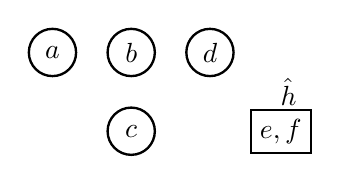
\begin{tikzpicture}
        % Singletons
        \def \ax{0}   \def \ay{0}
        \def \bx{1}   \def \by{0}
        \def \dx{2}   \def \dy{0}
        \def \cx{1}   \def \cy{-1}
        \def \hx{2.9}   \def \hy{-1}

        \draw[line width=0.3mm] (\ax, \ay) circle (0.3) node[anchor=center]{$a$};
        \draw[line width=0.3mm] (\bx, \by) circle (0.3) node[anchor=center]{$b$};
        \draw[line width=0.3mm] (\cx, \cy) circle (0.3) node[anchor=center]{$c$};
        \draw[line width=0.3mm] (\dx, \dy) circle (0.3) node[anchor=center]{$d$};
        % Cluster
        \node[rectangle, draw, line width=0.3mm] at (\hx, \hy) {$e,f$};
        \node at (\hx + 0.1, \hy + 0.5) {$\hat{h}$};

        % Attacks
        \DrawAttackDiagonal{NRL}{\hx}{\hy+0.1}{\dx}{\dy}
        \DrawAttackVertical{D}{\bx}{\by}{\cx}{\cy}
        \DrawAttackDiagonal{NRL}{\cx}{\cy}{\ax}{\ay}
        \DrawAttackHorizontal{L}{\dx}{\dy}{\bx}{\by}
        \DrawAttackHorizontal{L}{\bx}{\by}{\ax}{\ay}
    \end{tikzpicture}
    \caption{Concretized AF $\hat{F}'$ after Step 5}
    \label{example:algorithmConcretizeSingletonsStep5}
\end{figure}
\vspace{-0.2cm}

\begin{algorithm}[H]
    \caption{Concretizing Singletons Pseudocode Step 5}\label{alg:concretizingSingletonsStep5}
    \begin{algorithmic}[1]
        \Require $F: AF(A, R)$ \Comment{Concrete AF}
        \Require $\hat{F}: AF(\hat{A}, \hat{R})$ \Comment{Abstract AF}
        \Require $\hat{F}': AF(\hat{A}', \hat{R}')$ \Comment{Concretized Cluster}
        \Require $e: list(S)$ \Comment{Concretizer List}
        \For{$c_i$ in $\hat{F}'.clusters$}
            \If{$c_i.argAmount == 1$}
                \State $c_i \gets Singleton$
            \ElsIf{$c_i.argAmount == 0$}
                \State $\hat{F}'.remove(c_i)$
            \EndIf
        \EndFor
    \end{algorithmic}
\end{algorithm}


\newpage
\section{Computation of Concretizer List}
\label{sec:ComputationOfConcretizerList}
% Why do we need the algorithm
When talking about clustering AFs, faithfulness is an important property. If an AF is spurious, we find at least one extension, which cannot be mapped to a concrete extension. Based on the spurious extensions, we try to concretize the arguments of the abstract AF, to obtain faithfulness. This mutation is realized through the concretizer list.

% What is concretizer list
The concretizer list is a list of sets of clustered arguments. Each set is a unique combination of arguments, which are being concretized to find a faithful AF. All the sets of the concretizer list are attempted iteratively, where the order is dependent on the size of the set. We use a heuristic approach, putting the main focus on local changes. Here we operate directly on the arguments and its attackers which make a set spurious, instead of applying global changes to the AF. Further, a minimal deviation of the abstract AF is usually desired, so small concretizer sets are checked first.

% Input: spurious set
The input to the computation of the concretizer list is a set of the arguments of all the spurious extensions. 
As observed empirically, the computation intensity of the algorithm is highly dependent on the amount of attacks. If the arguments of the spurious set have many attackers or are attacking a lot of other arguments, we observe an exponential growth on the execution time.


% Example base
Let us have a look at an example to demonstrate how the concretizer list is computed. A concrete AF $G$ is defined in \cref{fig:AlgorithmCopmutationOfConcretizerListDouble}(a) and a corresponding abstract AF $\hat{G}$ in \cref{fig:AlgorithmCopmutationOfConcretizerListDouble}(b).


\vspace{0.3cm}
\begin{figure}[h]
    \begin{subfigure}[b]{0.475\textwidth}
    \centering
    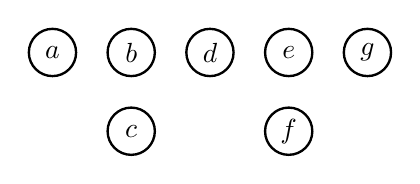
\begin{tikzpicture}
        % Singletons
        \def \ax{0}   \def \ay{0}
        \def \bx{1}   \def \by{0}
        \def \cx{1}   \def \cy{-1}
        \def \dx{2}   \def \dy{0}
        \def \ex{3}   \def \ey{0}
        \def \fx{3}   \def \fy{-1}
        \def \gx{4}   \def \gy{0}

        \draw[line width=0.3mm] (\ax, \ay) circle (0.3) node[anchor=center]{$a$};
        \draw[line width=0.3mm] (\bx, \by) circle (0.3) node[anchor=center]{$b$};
        \draw[line width=0.3mm] (\cx, \cy) circle (0.3) node[anchor=center]{$c$};
        \draw[line width=0.3mm] (\dx, \dy) circle (0.3) node[anchor=center]{$d$};
        \draw[line width=0.3mm] (\ex, \ey) circle (0.3) node[anchor=center]{$e$};
        \draw[line width=0.3mm] (\fx, \fy) circle (0.3) node[anchor=center]{$f$};
        \draw[line width=0.3mm] (\gx, \gy) circle (0.3) node[anchor=center]{$g$};

        % Attacks
        \DrawSelfAttackLeftSingleton{\ax}{\ay}
        \DrawAttackHorizontal{B}{\bx}{\by}{\ax}{\ay}
        \DrawAttackHorizontal{R}{\bx}{\by}{\dx}{\dy}
        \DrawAttackHorizontal{B}{\ex}{\ey}{\dx}{\dy}
        \DrawAttackHorizontal{R}{\ex}{\ey}{\gx}{\gy}
        \DrawAttackVertical{B}{\bx}{\by}{\cx}{\cy}
        \DrawAttackVertical{D}{\ex}{\ey}{\fx}{\fy}
        \DrawAttackDiagonal{PLR}{\fx}{\fy}{\gx}{\gy}
    \end{tikzpicture}
    \subcaption{Concrete AF $G$}
    \label{af:algorithmConcretizer1}
\end{subfigure}%
\begin{subfigure}[b]{0.475\textwidth}
    \centering
    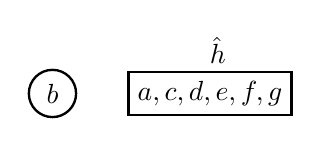
\begin{tikzpicture}
        % Singletons
        \def \bx{0}   \def \by{0}
        \def \hx{2}   \def \hy{0}

        \draw[line width=0.3mm] (\bx, \by) circle (0.3) node[anchor=center]{$b$};

        % Cluster
        \node[rectangle, draw, line width=0.3mm] at (\hx, \hy) {$a, c, d, e, f, g$};
        \node at (\hx + 0.1, \hy + 0.55) {$\hat{h}$};
        % Attacks
        \DrawAttackHorizontal{B}{\hx-0.85}{\hy}{\bx}{\by}
        \DrawSelfAttackRightTopCluster{\hx+1}{\hy+0.29}

    \end{tikzpicture}
    \subcaption{Abstract AF $\hat{G}$}
    \label{af:algorithmConcretizer2}
\end{subfigure}
\caption{Concrete and abstract AFs}
\label{fig:AlgorithmCopmutationOfConcretizerListDouble}
\end{figure}
\vspace{0.3cm}

If we have a look at the stable extensions of the concrete AF $G$, i.e.\ 
$stb(G) = \bigl\{\{b, c\}\bigl\}$ and at the abstractly stable extensions of the abstract AF $\hat{G}$, i.e.\ 
$\hat{stb}(G) = \bigl\{\{b, \hat{h}\}, \{\hat{h}\}, \{b\}\bigl\}$, we can see that the abstractly stable extensions $\{\hat{h}\}$ and $\{b\}$ are spurious. The input to the concretizer list computation is a collection of the arguments of all the spurious sets, which in this case is $\{b, \hat{h}\}$.

% Filter Cluster out of spurious set, because we cant concretize cluster
The first step is to filter out the clusters of the input, since clusters are not present in the concrete AF and therefore do not attack any singletons and are not being attacked. So we reduce the concretizer list from $\{b, \hat{h}\}$ to $\{b\}$.

% Get combination as defender depth 2
Next, we have a look at the neighbouring arguments of the current concretizer list.  Neighbours in this context are arguments which attack, or are being attacked by an argument. The depth defines how many arguments are between the attacks. A depth of $1$ represents the direct attacker of an argument and the arguments, which are being attacked by the argument. A depth $2$ argument is an argument, which has some attack relation (e.g.\ attacks the argument or is attacked by the argument) with a depth $1$ argument. Some arguments can have multiple depths (e.g.\ argument $c$. It is a direct attacker of the argument $b$ with depth $0$, but also a direct attacker of the argument $c$ with depth $1$), then the lower depth is chosen as the representative.

We used a search depth of $2$ in our implementation. So when having a look at our example, we take the defender of depth $1$ and $2$, in \cref{af:algorithmConcretizer3} depicted in dotted line style and the attacker, depicted in dashed line style. The pseudo-code of this procedure is listed in \cref{alg:concretizerListNeighbours} where $N$ represents the list of neighbours at depth $2$ that we are computing. Furthermore, the function $neighbours(arg)$ returns all the direct neighbours of the argument $arg$.



%Depth 2 Attacker
\vspace{0.1cm}
\begin{figure}[h!]
    \centering
    \begin{tikzpicture}
        % Singletons
        \def \ax{0}   \def \ay{0}
        \def \bx{1}   \def \by{0}
        \def \cx{1}   \def \cy{-1}
        \def \dx{2}   \def \dy{0}
        \def \ex{3}   \def \ey{0}
        \def \fx{3}   \def \fy{-1}
        \def \gx{4}   \def \gy{0}

        \draw[line width=0.3mm] (\ax, \ay) circle (0.3) node[anchor=center]{$a$};
        \draw[c2, densely dotted, line width=0.3mm] (\ax,\ay) circle (0.4);
        \node[text=c2] at (\ax+0.33, \ay+0.45) {\footnotesize 1};

        \draw[line width=0.3mm] (\bx, \by) circle (0.3) node[anchor=center]{$b$};
        \draw[c3] (\bx,\by) circle (0.4);
        \node[text=c3] at (\bx+0.33, \by+0.45) {\footnotesize 0};

        \draw[line width=0.3mm] (\cx, \cy) circle (0.3) node[anchor=center]{$c$};
        \draw[c2, densely dotted, line width=0.3mm] (\cx,\cy) circle (0.4);
        \node[text=c2] at (\cx+0.55, \cy) {\footnotesize 1};

        \draw[line width=0.3mm] (\dx, \dy) circle (0.3) node[anchor=center]{$d$};
        \draw[c1, densely dashed] (\dx,\dy) circle (0.4);
        \node[text=c1] at (\dx+0.33, \dy+0.45) {\footnotesize 1};

        \draw[line width=0.3mm] (\ex, \ey) circle (0.3) node[anchor=center]{$e$};
        \draw[c1, densely dashed] (\ex,\ey) circle (0.4);
        \node[text=c1] at (\ex+0.33, \ey+0.45) {\footnotesize 2};

        \draw[line width=0.3mm] (\fx, \fy) circle (0.3) node[anchor=center]{$f$};
        \node at (\fx+0.45, \fy) {\footnotesize 3};

        \draw[line width=0.3mm] (\gx, \gy) circle (0.3) node[anchor=center]{$g$};
        \node at (\gx+0.33, \gy+0.45) {\footnotesize 3};

        % Attacks
        \DrawSelfAttackLeftSingleton{\ax}{\ay}
        \DrawSelfAttackLeftSingleton{\cx}{\cy}
        \DrawAttackHorizontal{B}{\bx}{\by}{\ax}{\ay}
        \DrawAttackHorizontal{R}{\bx}{\by}{\dx}{\dy}
        \DrawAttackHorizontal{B}{\ex}{\ey}{\dx}{\dy}
        \DrawAttackHorizontal{R}{\ex}{\ey}{\gx}{\gy}
        \DrawAttackVertical{B}{\bx}{\by}{\cx}{\cy}
        \DrawAttackVertical{D}{\ex}{\ey}{\fx}{\fy}
        \DrawAttackDiagonal{PLR}{\fx}{\fy}{\gx}{\gy}
    \end{tikzpicture}
    \caption{Depth of singletons from the perspective of $b$}
    \label{af:algorithmConcretizer3}
\end{figure}
\vspace{-0.2cm}

\begin{algorithm}
    \caption{Computation of Concretizer list Algorithm: Neighbours}\label{alg:concretizerListNeighbours}
    \begin{algorithmic}[1]
        \Require $G: AF(A, R)$ \Comment{Concrete AF}
        \Require $s: list(Arguments)$ \Comment{Working List}
        \State $N$ $\gets$ $\emptyset$ \Comment{$N$ = list of neighbours}
        \State $n(1) \gets \emptyset$ \Comment{List of neighbours with depth 1}
        \For{$s_i$ in $s$} \Comment{Get neighbours}
            \For{$n$ in $neighbours(s_i)$} \Comment{depth 1 attacker}
                \State $n(1).append(n)$
                \State $N.append(n)$
            \EndFor
            \For{$n(1)_i$ in $n(1)$}
                \For{$n$ in $neighbours(n(1)_i)$} \Comment{depth 2 attacker}
                    \State $N.append(n)$
                \EndFor
            \EndFor
        \EndFor
    \end{algorithmic}
\end{algorithm}


Now the concretizer list is expanded with all the possible combinations of the neighbours. The neighbours of the current example are $\{a, c, d, e\}$. When building the combinations, we create the table defined in \cref{table:algorithmConcretizer1}.

\begin{table}[htb]
    \centering
    \caption{Combinations of $\{a, c, d, e\}$}
    \begin{tabular}{ |c|c|c|c| }
     \hline
     size $1$ & size $2$ & size $3$ & size $4$\\
     \hline
     \hline
     $\{a\}$ & $\{a, c\}$ & $\{a, c, d\}$ &$\{a, c, d, e\}$ \\
     \hline
     $\{c\}$ & $\{a, d\}$ & $\{a, d, e\}$ & \\
     \hline
     $\{d\}$ & $\{c, d\}$ & $\{c, d, e\}$ & \\
     \hline
      & $\{d, e\}$ &  & \\
     \hline
       &  &  & \\
     \hline
       &  &  & \\
     \hline
    \end{tabular}
\label{table:algorithmConcretizer1}
\end{table}

The combination table grows exponentially to the base of 2. Therefore, the size of the neighbours is crucial. If we have too many neighbours, the computation would need too much memory and turns infeasible to compute.

% Add concretizer list defined by the user
% deduplicate
If the user has provided arguments which have to be concretized as program argument, we add them to each combination set. After adding them, we filter for duplicates to keep the concretizer list size to a minimum.

% Filter singletons which are not in cluster, because cant concretize singletons
% deduplicate
Next, we need to filter out the arguments, which are not in clusters, since singletons are already concrete. This filtering could lead to some duplicates again, which we need to remove once again to minimize the memory consumption and reduce the amount of faitfhul checks. In our example, we remove the set $\{b\}$.

Finally, we sort the list by the set size and return it. In the current example we would return the whole table, because no concretizer arguments were provided by the user. So the concretizer list would be
$\bigl\{\{a\}$
$\{c\}$
$\{d\}$
$\{a, c\}$
$\{a, d\}$
$\{c, d\}$
$\{d, e\}$
$\{a, c, d\}$
$\{a, d, e\}$
$\{c, d, e\}$
$\{a, c, d, e\}\bigl\}$. The pseudo-code for the last step is stated in \cref{alg:concretizerListCombinationAndCleanup}.


\begin{algorithm}
    \caption{Computation of Concretizer list Algorithm: Combinations and Cleanup}\label{alg:concretizerListCombinationAndCleanup}
    \begin{algorithmic}[1]
        \Require $G: AF(a_1, r_1)$ \Comment{Concrete AF}
        \Require $\hat{G}: AF(a_2, r_2)$ \Comment{Abstract AF}
        \Require $s: list(Arguments)$ \Comment{Working List}
        \Require $ca: list(Arguments)$ \Comment{Concretize arguments parameter}

        \State $C \gets$ combinations of N with $range(1, len(N)-1)$ \Comment{Combination List}

        \For{$ca_i$ in $ca$} \Comment{Parameter Arguments to be concretized}
            \For{$c_i$ in $C$}
                \State $c_i.append(ca_i)$
            \EndFor
        \EndFor
        \State $C.deduplicate()$

        \For{$s_i$ in $C$} \Comment{Remove clusters}
            \For{$a_i$ in $s_i$}
                \If{$\hat{G}[a_i]$ is cluster}
                    \State $s_i.remove(a_i)$
                \EndIf
            \EndFor
        \EndFor
        \State \Return $s.sortBySize()$
    \end{algorithmic}
\end{algorithm}

\newpage

\section{Finding Faithful Clusterings}
\label{sec:AlgorithmicApproachToComputeFaifthulClusterings}
When clustering AFs, information gets lost. If crucial information is abstracted in a way, s.t.\ we can draw erroneous conclusions, we have a spurious AF. Spurious abstract AFs do not represent the corresponding concrete AFs. Thus, we need to transform the abstract AF, s.t.\ only correct solutions can be drawn, which we then call faithful. The algorithm we designed, takes as input a concrete AF denoted to $G$, and an abstract AF $\hat{G}$. First we determine, if the abstract AF $\hat{G}$ is spurious, by calculating the semantics extensions and attempting to find spurious set. If no spurious set can be found, the AF is faithful and no further mutations are needed.

But if we find spurious extensions, we build the concretizer list as specified previously in \cref{sec:ComputationOfConcretizerList}. Recall, that the concretizer list operates with the depth of neighbours of $2$. This means, that depending on the AF, we can not guarantee to find a faithful AF. If the spurious extension of an AF $G$ has an argument $a$ with depth 3 to an argument $b$, and the only faithful AF is the concrete one, then we will not find the faithful AF.

Finally, we concretize the concretizer list set after set and check for faithfulness. The algorithm is listed in \cref{alg:computeFaithfulClusters}.



\begin{example}
    Let us have a look at an example and define an AF $G=(A,R)$ with the arguments $A=\{a, b, c, d, e, f\}$ and the attacks $R=\bigl\{(a, a)$, $(a, c),$ $(b, a),$ $(c, b),$ $(c, d),$ $(d, c),$ $(e, b),$ $(b, e),$ $(f, f)\bigl\}$, depicted in \cref{fig:AlgorhtmAlgorithmicApproachCopmuteFaithfulClusteringDouble}(a). When clustering the arguments $\{a, b, f\}$ we obtain the abstract AF $\hat{G}=(\hat{A}, \hat{R})$ depicted in \cref{fig:AlgorhtmAlgorithmicApproachCopmuteFaithfulClusteringDouble}(b). Where the arguments are $\hat{A}=\{c, d, e, \hat{h}\}$. The attacks of the abstract AF are $\hat{R}=\{(\hat{h},$ $\hat{h}),$ $(\hat{h}, c),$ $(c, d),$ $(d, c),$ $(\hat{h}, e),$ $(e, \hat{h})\}$ and the cluster $\hat{h}$ contains the arguments $\{a, b, f\}$.
\end{example}

\vspace{0.3cm}
\begin{figure}[h]
    \centering
    \begin{subfigure}[t]{0.45\textwidth}
    \centering
    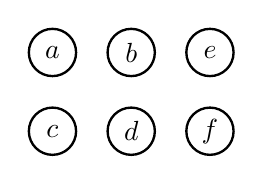
\begin{tikzpicture}
        % Singletons
        \def \ax{0}   \def \ay{0}
        \def \bx{1}   \def \by{0}
        \def \cx{0}   \def \cy{-1}
        \def \dx{1}   \def \dy{-1}
        \def \ex{2}   \def \ey{0}
        \def \fx{2}   \def \fy{-1}

        \draw[line width=0.3mm] (\ax, \ay) circle (0.3) node[anchor=center]{$a$};
        \draw[line width=0.3mm] (\bx, \by) circle (0.3) node[anchor=center]{$b$};
        \draw[line width=0.3mm] (\cx, \cy) circle (0.3) node[anchor=center]{$c$};
        \draw[line width=0.3mm] (\dx, \dy) circle (0.3) node[anchor=center]{$d$};
        \draw[line width=0.3mm] (\ex, \ey) circle (0.3) node[anchor=center]{$e$};
        \draw[line width=0.3mm] (\fx, \fy) circle (0.3) node[anchor=center]{$f$};

        % Attacks
        \DrawSelfAttackLeftSingleton{\ax}{\ay}
        \DrawAttackVertical{D}{\ax}{\ay}{\cx}{\cy}
        \DrawAttackHorizontal{L}{\bx}{\by}{\ax}{\ay}
        \DrawAttackDiagonal{PLR}{\cx}{\cy}{\bx}{\by}
        \DrawAttackHorizontal{B}{\dx}{\dy}{\cx}{\cy}
        \DrawAttackHorizontal{B}{\ex}{\ey}{\bx}{\by}
        \DrawSelfAttackRightSingleton{\fx}{\fy}
    \end{tikzpicture}
    \subcaption{Concrete AF $G$}
    \label{af:computeFaithfulCluster1a}
\end{subfigure}%
\begin{subfigure}[t]{0.45\textwidth}
    \centering
    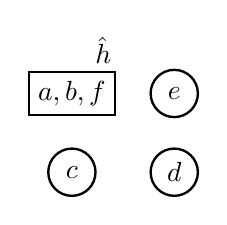
\begin{tikzpicture}
        % Singletons
        \def \cx{0}   \def \cy{-1}
        \def \dx{1.3}   \def \dy{-1}
        \def \ex{1.3}   \def \ey{0}
        \def \hx{0}   \def \hy{0}

        \draw[line width=0.3mm] (\cx, \cy) circle (0.3) node[anchor=center]{$c$};
        \draw[line width=0.3mm] (\dx, \dy) circle (0.3) node[anchor=center]{$d$};
        \draw[line width=0.3mm] (\ex, \ey) circle (0.3) node[anchor=center]{$e$};

        % Cluster
        \node[rectangle, draw, line width=0.3mm] at (\hx, \hy) {$a, b, f$};
        \node at (\hx + 0.4, \hy + 0.55) {$\hat{h}$};
        % Attacks
        \DrawSelfAttackLeftTopCluster{\hx-0.45}{\hy+0.29}
        \DrawAttackVertical{D}{\hx}{\hy}{\cx}{\cy}
        \DrawAttackHorizontal{B}{\dx}{\dy}{\cx}{\cy}
        \DrawAttackHorizontal{B}{\ex}{\ey}{\hx+0.3}{\hy}

    \end{tikzpicture}
    \subcaption{Abstract AF $\hat{G}$}
    \label{af:computeFaithfulCluster1b}
\end{subfigure}
\caption{Concrete and abstract AF}
\label{fig:AlgorhtmAlgorithmicApproachCopmuteFaithfulClusteringDouble}
\end{figure}
\vspace{0.3cm}


When taking a look at the conflict-free sets of the concrete AF $G$ (i.e.\ $\bigl\{ \emptyset,$ $\{b\},$ $\{c\},$ $\{d\},$ $\{e\},$ $\{b, d\},$  $\{c, e\},$ $\{d, e\} \bigl\}$) and the abstractly conflict-free sets of the abstract AF $\hat{G}$ (e.g.\ $\bigl\{ \emptyset,$ $\{c\},$ $\{d\},$ $\{e\},$ $\{\hat{h}\},$ $\{c, e\},$ $\{c, \hat{h}\},$ $\{d, e\},$ $\{d, \hat{h}\},$ $\{e, \hat{h}\},$ $\{c, e, \hat{h}\},$ $\{e, d, \hat{h}\} \bigl\}$) we can observe, that the abstract AF $\hat{G}$ is spurious due to the sets $\bigl\{\{\hat{h}, d, e\},$ $\{\hat{h}, e\},$ $\{c, \hat{h}, e\},$ $\{c, \hat{h}\}\bigl\}$. Now we compute the concretizer list and obtain the sets $\bigl\{ \{a\}, \{b\}, \{a, b\}\bigl\}$. In this example, the only faithful solution we can obtain by concretizing is the concrete AF $G$. Thus, concretizing the set $\{a, b\}$ leads to a faithful AF.
\vspace{0.5cm}

\begin{algorithm}
    \caption{Compute Faithful Clusters}\label{alg:computeFaithfulClusters}
    \begin{algorithmic}[1]
        \Require $G: AF(A, R)$ \Comment{Concrete AF}
        \Require $\hat{G}: AF(\hat{A}, \hat{R})$ \Comment{Abstract AF}
        \State $sp \gets computeSpuriousExtensions(G, \hat{G})$
        \State $conc \gets computeConcretizerList(sp)$
        \For{$set_i$ in $sp$}
            \State $\hat{G}' \gets concretize(\hat{G}, set_i)$
            \If{$checkFaithfulness(G, \hat{G}')$}
                \State \Return $\hat{G}'$
            \EndIf
        \EndFor
    \end{algorithmic}
\end{algorithm}



\newpage
\section{Heuristics and Refinements}
\label{sec:HeuristicsAndRefinements}

To speed up the process of computing semantics extensions, we came up with heuristics and refinements to improve the faithful/spurious check of two AFs for admissible and stable semantics and for conflict-free the general approach of finding semantics sets. Some heuristics were already mentioned previously, like sorting the concretizer list by size to obtain a rather small mutation of the spurious AF. But we also implemented shortcuts and refinements, specific for every semantics.

\paragraph{Conflict-free} Let us begin with a refinement for the conflict-free sets computation. When computing a single conflict-free set, with the amount of arguments greater than 1, we extract every subset, which is conflict-free as well. Formally, if $X$ is a conflict-free set and $|X|\geq 2$, then $\forall S \subseteq X$, $S$ is conflict-free. This property can be derived from the definition of conflict-free sets. Recall that a set of (clustered) arguments is conflict-free if there is no attack between singletons in the set. Thus, if there are no attacks between the arguments in $X$, and $S \subseteq X$, we can conclude that there are no attacks between the argument in $S$. With this adaption we can speed up the process of generating conflict-free sets, which is also used in the faithful/spurious check.

\paragraph{Admissible} Next, we will define the refinements made for the admissible semantics. Other than conflict-free sets, for (abstract) admissible sets we cannot derive directly information from the subsets. But we can decrease the computation time of showing spuriousness or faithfulness by adding the negated admissible formula for the concrete AF. This removes the faithful admissible sets, which are composed of only singletons and can therefore be directly mapped from the abstract admissible sets to the concrete ones. The remaining sets to be computed are the spurious sets, or abstract admissible sets containing at least one cluster (since the concrete AF does not possess clusters and are therefore not ignored).

Recall, that a set of arguments is abstractly admissible, if it is abstractly conflict-free and if every singleton which is being attacked, has a defender. We refine the formula from \cref{def:booleanFormulaAdmissible}, denoted as $\varphi_{adm}$ with the refinement denoted as $\eta_{adm}$.


$$
    \hat{adm}=\ \varphi_{adm}(\hat{F}) \land \eta_{adm}(F)
$$


Where $\eta_{adm}(F)$ is defined as the negated admissible formula of the concrete AF.


$$
    \eta_{adm}(F)=\ \overline{cf}(F) \lor \overline{def}(F)
$$


The two new introduced components (i.e.\ $\overline{cf}$ and $\overline{def}$) define together the refinement. Here, $\overline{cf}$ stands for the negated part of the conflict-free sets from the concrete AF and $\overline{def}$ defines that we want to ignore all the sets from the concrete AF which are defending themselves from an attack.

\begin{align*}
    \overline{cf}(F)&=\ \bigvee_{a \in A_{\mathit{Single}}} \big( \bigvee_{b:(b,a)\in R, b \in A_{\mathit{Single}}} \big( a \land b \big) \big)\\
    \overline{def}(F)&=\ \big( \bigvee_{a \in A_{\mathit{Single}}}\big( a \land \bigvee_{b:(b,a)\in R} \big( \bigwedge_{c:(c, b)\in R} \lnot c\big)\big) \big)
\end{align*}

\paragraph{Stable} For the stable semantics we apply the same principle as for abstract admissibility. Since we cannot conclude anything from the subsets of the computed (abstract) semantics, we need to add the negation of the stable formula for the concrete AF. With this, we aim to reduce the semantics extensions which need to be computed for showing spuriousness or faithfulness, without losing crucial information. The eliminated abstract extensions are simply the extensions, which can be directly mapped to the concrete stable extensions. The remaining extensions that need to be computed are either spurious extensions, or extensions which have at least one cluster and need to be expanded and checked separately for spuriousness. Recall, that a set of
arguments is abstractly stable, if it is abstractly conflict-free and if an argument is not in the abstractly stable extension, it implies that an argument in the abstractly stable extension is attacking it. Furthermore if the abstractly stable extension is not attacking an argument, then every singleton attacking the argument is not in the abstractly stable extension. We refine this formula from \cref{def:booleanFormulaStable}, denoted as $\varphi_{stb}$ with the refinement denoted as $\eta_{stb}$.


$$ \hat{stb}=\  \varphi_{stb}(\hat{F}) \land \eta_{stb}(F) $$

\vspace{0.04cm}
Here $\eta_{stb}$ is defined as the negated stable formula of the concrete AF.
\vspace{0.01cm}


$$
\eta_{stb}(F) =\ \overline{cf}(F) \lor \overline{att}(F)
$$


The two components (i.e.\ $\overline{cf}$, $\overline{att}$) represent two different conditions which together define the refinement. Here, $\overline{cf}$ is the negated part of conflict-freeness of the concrete AF and $\overline{att}$ describes that we want to ignore the concrete stable sets which impliy that if and argument being outside the stable set, has an attacker inside the stable set.

\begin{align*}
    \overline{cf}(F)&=\ \bigvee_{a \in A_{\mathit{Single}}} \big( \bigvee_{b:(b,a)\in R, b \in A_{\mathit{Single}}} \big( a \land b \big) \big)\\[0.2cm]
    \overline{att}(F)&=\ \bigvee_{a \in A} \big( \lnot a \bigwedge_{b:(b,a)\in R} \lnot b \big)
\end{align*}


\section{Relations between Spurious Sets }
\label{sec:AlgorithmsRelationsBetweenSpuriousSets}

When developing the tool, we came up with different theories. Some theories were discarded immediately, some were implemented (recall \cref{sec:HeuristicsAndRefinements}) and others had to be proven wrong. This section describes the most promising assumptions which turned out to be wrong.

We came up with the theory, that every subset of a stable spurious extension, is spurious as well. Formally, if $S$ is a spurious stable set of the abstract AF $\hat{G}$. Then for every subset $T \subseteq S$, $T$ is spurious as well. This would reduce the computation time of finding spurious sets drastically. Unfortunately, we can disprove this theory with a counter-example.

\begin{example}
    Let us define $G=(A,R)$ to be a concrete AF, with the arguments $A=\{a, b, c, d, e, f\}$ and the attacks $R=\bigl\{ (b, a)$, $(a, d)$, $(a, c)$, $(c, e)$, $(c, f)$, $(d, f) \bigl\}$ depicted in \cref{fig:AlgorithmRefutedTheoryDefinition}(a). The spurious abstract AF $\hat{G}=(\hat{A}, \hat{R})$ is defined by the arguments $\hat{A}=\{\hat{g}, e\}$, with the cluster $\hat{g}$ containing the arguments $\{a, b, c, d, f\}$ and the attacks being $\hat{R}=\bigl\{(\hat{g}, \hat{g}), (\hat{g}, e)\bigl\}$ depicted in \cref{fig:AlgorithmRefutedTheoryDefinition}(b).

\vspace{0.3cm}
\begin{figure}[h]
    \centering
    \begin{subfigure}[t]{0.45\textwidth}
        \centering
        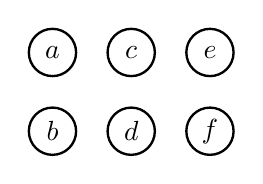
\begin{tikzpicture}
            \def \ax{0}   \def \ay{0}
            \def \bx{0}   \def \by{-1}
            \def \cx{1}   \def \cy{0}
            \def \dx{1}   \def \dy{-1}
            \def \ex{2}   \def \ey{0}
            \def \fx{2}   \def \fy{-1}

            \draw[line width=0.3mm] (\ax, \ay) circle (0.3) node[anchor=center]{$a$};
            \draw[line width=0.3mm] (\bx, \by) circle (0.3) node[anchor=center]{$b$};
            \draw[line width=0.3mm] (\cx, \cy) circle (0.3) node[anchor=center]{$c$};
            \draw[line width=0.3mm] (\dx, \dy) circle (0.3) node[anchor=center]{$d$};
            \draw[line width=0.3mm] (\ex, \ey) circle (0.3) node[anchor=center]{$e$};
            \draw[line width=0.3mm] (\fx, \fy) circle (0.3) node[anchor=center]{$f$};
            % Attacks
            \DrawAttackHorizontal{R}{\ax}{\ay}{\cx}{\cy}
            \DrawAttackHorizontal{R}{\cx}{\cy}{\ex}{\ey}
            \DrawAttackHorizontal{R}{\dx}{\dy}{\fx}{\fy}
            \DrawAttackVertical{U}{\bx}{\by}{\ax}{\ay}
            \DrawAttackDiagonal{NLR}{\ax}{\ay}{\dx}{\dy}
            \DrawAttackDiagonal{NLR}{\cx}{\cy}{\fx}{\fy}
        \end{tikzpicture}
        \subcaption{Concrete AF}
        \label{af:implementationRefutedTheoryA}
    \end{subfigure}
    \begin{subfigure}[t]{0.45\textwidth}
    \centering
    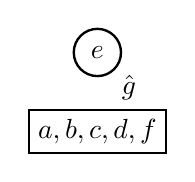
\begin{tikzpicture}
        \def \ex{0}   \def \ey{0}
        \def \gx{0}   \def \gy{-1}

        \draw[line width=0.3mm] (\ex, \ey) circle (0.3) node[anchor=center]{$e$};
        \node[rectangle, draw, line width=0.3mm] at (\gx, \gy) {$a, b, c, d, f$};
        \node at (\gx + 0.4, \gy+0.55) {$\hat{g}$};
        % Attacks
        \DrawSelfAttackLeftTopCluster{\gx-0.8}{\gy+0.3}
        \DrawAttackVertical{U}{\gx}{\gy}{\ex}{\ey}

    \end{tikzpicture}
    \subcaption{Spurious abstract AF}
    \label{af:implementationRefutedTheoryB}
    \end{subfigure}%
\caption{Concrete and spurious abstract AF}
\label{fig:AlgorithmRefutedTheoryDefinition}
\end{figure}
\vspace{0.3cm}

When computing the stable extensions of $G$, we obtain $\bigl\{b, c, d\bigl\}$, for the abstract AF $\hat{G}$ we get the abstractly stable extensions $\big\{\{\hat{g}\}, \{\hat{g}, e\}\big\}$. Since the abstractly stable extension $\{\hat{g}, e\}$ is spurious, we have a spurious abstract AF. Now, we can have a look at the subsets of the spurious extensions and check if every subset is spurious as well. When trying to map a subset of $\{\hat{g}, e\}$, e.g.\ $\{\hat{g}\}$ to the concrete extension $\{b, c, d\}$, we can see that it is faithful. Thus, we found a subset of a spurious extension, which is not spurious.
\end{example}